\documentclass[twoside]{book}

% Packages required by doxygen
\usepackage{calc}
\usepackage{doxygen}
\usepackage{graphicx}
\usepackage[utf8]{inputenc}
\usepackage{makeidx}
\usepackage{multicol}
\usepackage{multirow}
\usepackage{textcomp}
\usepackage[table]{xcolor}

% Font selection
\usepackage[T1]{fontenc}
\usepackage{mathptmx}
\usepackage[scaled=.90]{helvet}
\usepackage{courier}
\usepackage{amssymb}
\usepackage{sectsty}
\renewcommand{\familydefault}{\sfdefault}
\allsectionsfont{%
  \fontseries{bc}\selectfont%
  \color{darkgray}%
}
\renewcommand{\DoxyLabelFont}{%
  \fontseries{bc}\selectfont%
  \color{darkgray}%
}

% Page & text layout
\usepackage{geometry}
\geometry{%
  a4paper,%
  top=2.5cm,%
  bottom=2.5cm,%
  left=2.5cm,%
  right=2.5cm%
}
\tolerance=750
\hfuzz=15pt
\hbadness=750
\setlength{\emergencystretch}{15pt}
\setlength{\parindent}{0cm}
\setlength{\parskip}{0.2cm}
\makeatletter
\renewcommand{\paragraph}{%
  \@startsection{paragraph}{4}{0ex}{-1.0ex}{1.0ex}{%
    \normalfont\normalsize\bfseries\SS@parafont%
  }%
}
\renewcommand{\subparagraph}{%
  \@startsection{subparagraph}{5}{0ex}{-1.0ex}{1.0ex}{%
    \normalfont\normalsize\bfseries\SS@subparafont%
  }%
}
\makeatother

% Headers & footers
\usepackage{fancyhdr}
\pagestyle{fancyplain}
\fancyhead[LE]{\fancyplain{}{\bfseries\thepage}}
\fancyhead[CE]{\fancyplain{}{}}
\fancyhead[RE]{\fancyplain{}{\bfseries\leftmark}}
\fancyhead[LO]{\fancyplain{}{\bfseries\rightmark}}
\fancyhead[CO]{\fancyplain{}{}}
\fancyhead[RO]{\fancyplain{}{\bfseries\thepage}}
\fancyfoot[LE]{\fancyplain{}{}}
\fancyfoot[CE]{\fancyplain{}{}}
\fancyfoot[RE]{\fancyplain{}{\bfseries\scriptsize Generated on Wed Jun 29 2016 11\-:01\-:14 for Hi\-Q\-P\-\_\-\-Controllers R\-O\-S Package by Doxygen }}
\fancyfoot[LO]{\fancyplain{}{\bfseries\scriptsize Generated on Wed Jun 29 2016 11\-:01\-:14 for Hi\-Q\-P\-\_\-\-Controllers R\-O\-S Package by Doxygen }}
\fancyfoot[CO]{\fancyplain{}{}}
\fancyfoot[RO]{\fancyplain{}{}}
\renewcommand{\footrulewidth}{0.4pt}
\renewcommand{\chaptermark}[1]{%
  \markboth{#1}{}%
}
\renewcommand{\sectionmark}[1]{%
  \markright{\thesection\ #1}%
}

% Indices & bibliography
\usepackage{natbib}
\usepackage[titles]{tocloft}
\setcounter{tocdepth}{3}
\setcounter{secnumdepth}{5}
\makeindex

% Hyperlinks (required, but should be loaded last)
\usepackage{ifpdf}
\ifpdf
  \usepackage[pdftex,pagebackref=true]{hyperref}
\else
  \usepackage[ps2pdf,pagebackref=true]{hyperref}
\fi
\hypersetup{%
  colorlinks=true,%
  linkcolor=blue,%
  citecolor=blue,%
  unicode%
}

% Custom commands
\newcommand{\clearemptydoublepage}{%
  \newpage{\pagestyle{empty}\cleardoublepage}%
}


%===== C O N T E N T S =====

\begin{document}

% Titlepage & ToC
\hypersetup{pageanchor=false}
\pagenumbering{roman}
\begin{titlepage}
\vspace*{7cm}
\begin{center}%
{\Large Hi\-Q\-P\-\_\-\-Controllers R\-O\-S Package }\\
\vspace*{1cm}
{\large Generated by Doxygen 1.8.6}\\
\vspace*{0.5cm}
{\small Wed Jun 29 2016 11:01:14}\\
\end{center}
\end{titlepage}
\clearemptydoublepage
\tableofcontents
\clearemptydoublepage
\pagenumbering{arabic}
\hypersetup{pageanchor=true}

%--- Begin generated contents ---
\chapter{Namespace Index}
\section{Namespace List}
Here is a list of all documented namespaces with brief descriptions\-:\begin{DoxyCompactList}
\item\contentsline{section}{\hyperlink{namespacehiqp}{hiqp} }{\pageref{namespacehiqp}}{}
\end{DoxyCompactList}

\chapter{Hierarchical Index}
\section{Class Hierarchy}
This inheritance list is sorted roughly, but not completely, alphabetically\-:\begin{DoxyCompactList}
\item Joint\-Velocity\-Controller\begin{DoxyCompactList}
\item \contentsline{section}{hiqp\-:\-:Hi\-Q\-P\-\_\-\-Kinematic\-\_\-\-Controller}{\pageref{classhiqp_1_1HiQP__Kinematic__Controller}}{}
\end{DoxyCompactList}
\item \contentsline{section}{hiqp\-:\-:Task}{\pageref{classhiqp_1_1Task}}{}
\item \contentsline{section}{hiqp\-:\-:Task\-Manager}{\pageref{classhiqp_1_1TaskManager}}{}
\end{DoxyCompactList}

\chapter{Class Index}
\section{Class List}
Here are the classes, structs, unions and interfaces with brief descriptions\-:\begin{DoxyCompactList}
\item\contentsline{section}{\hyperlink{classhiqp_1_1HiQP__Kinematic__Controller}{hiqp\-::\-Hi\-Q\-P\-\_\-\-Kinematic\-\_\-\-Controller} \\*This is my awesome controller }{\pageref{classhiqp_1_1HiQP__Kinematic__Controller}}{}
\end{DoxyCompactList}

\chapter{File Index}
\section{File List}
Here is a list of all documented files with brief descriptions\-:\begin{DoxyCompactList}
\item\contentsline{section}{include/hiqp/\hyperlink{hiqp__kinematic__controller_8h}{hiqp\-\_\-kinematic\-\_\-controller.\-h} \\*Brief description of file }{\pageref{hiqp__kinematic__controller_8h}}{}
\item\contentsline{section}{include/hiqp/\hyperlink{hiqp__utils_8h}{hiqp\-\_\-utils.\-h} \\*Brief description of file }{\pageref{hiqp__utils_8h}}{}
\item\contentsline{section}{include/hiqp/\hyperlink{task_8h}{task.\-h} \\*Brief description of file }{\pageref{task_8h}}{}
\item\contentsline{section}{include/hiqp/\hyperlink{task__beh__fo_8h}{task\-\_\-beh\-\_\-fo.\-h} \\*Brief description of file }{\pageref{task__beh__fo_8h}}{}
\item\contentsline{section}{include/hiqp/\hyperlink{task__behaviour_8h}{task\-\_\-behaviour.\-h} \\*Brief description of file }{\pageref{task__behaviour_8h}}{}
\item\contentsline{section}{include/hiqp/\hyperlink{task__manager_8h}{task\-\_\-manager.\-h} \\*Brief description of file }{\pageref{task__manager_8h}}{}
\item\contentsline{section}{include/hiqp/\hyperlink{task__pop_8h}{task\-\_\-pop.\-h} \\*Brief description of file }{\pageref{task__pop_8h}}{}
\item\contentsline{section}{include/hiqp/\hyperlink{task__visualizer_8h}{task\-\_\-visualizer.\-h} \\*Brief description of file }{\pageref{task__visualizer_8h}}{}
\item\contentsline{section}{src/\hyperlink{hiqp__kinematic__controller_8cpp}{hiqp\-\_\-kinematic\-\_\-controller.\-cpp} \\*Brief description of file }{\pageref{hiqp__kinematic__controller_8cpp}}{}
\item\contentsline{section}{src/\hyperlink{hiqp__utils_8cpp}{hiqp\-\_\-utils.\-cpp} \\*Brief description of file }{\pageref{hiqp__utils_8cpp}}{}
\item\contentsline{section}{src/\hyperlink{task__beh__fo_8cpp}{task\-\_\-beh\-\_\-fo.\-cpp} \\*Brief description of file }{\pageref{task__beh__fo_8cpp}}{}
\item\contentsline{section}{src/\hyperlink{task__manager_8cpp}{task\-\_\-manager.\-cpp} \\*Brief description of file }{\pageref{task__manager_8cpp}}{}
\item\contentsline{section}{src/\hyperlink{task__pop_8cpp}{task\-\_\-pop.\-cpp} \\*Brief description of file }{\pageref{task__pop_8cpp}}{}
\item\contentsline{section}{src/\hyperlink{task__visualizer_8cpp}{task\-\_\-visualizer.\-cpp} \\*Brief description of file }{\pageref{task__visualizer_8cpp}}{}
\end{DoxyCompactList}

\chapter{Namespace Documentation}
\hypertarget{namespacehiqp}{\section{hiqp Namespace Reference}
\label{namespacehiqp}\index{hiqp@{hiqp}}
}
\subsection*{Classes}
\begin{DoxyCompactItemize}
\item 
struct \hyperlink{structhiqp_1_1HiQPStage}{Hi\-Q\-P\-Stage}
\item 
class \hyperlink{classhiqp_1_1HiQPSolver}{Hi\-Q\-P\-Solver}
\item 
class \hyperlink{classhiqp_1_1HiQPTimePoint}{Hi\-Q\-P\-Time\-Point}
\begin{DoxyCompactList}\small\item\em The time type used in this framework. \end{DoxyCompactList}\item 
class \hyperlink{classhiqp_1_1ROSDynamicsController}{R\-O\-S\-Dynamics\-Controller}
\begin{DoxyCompactList}\small\item\em This is my awesome controller. \end{DoxyCompactList}\item 
class \hyperlink{classhiqp_1_1ROSKinematicsController}{R\-O\-S\-Kinematics\-Controller}
\item 
class \hyperlink{classhiqp_1_1ROSTopicSubscriber}{R\-O\-S\-Topic\-Subscriber}
\item 
class \hyperlink{classhiqp_1_1ROSVisualizer}{R\-O\-S\-Visualizer}
\item 
class \hyperlink{classhiqp_1_1CasADiSolver}{Cas\-A\-Di\-Solver}
\item 
class \hyperlink{classhiqp_1_1TaskDynamics}{Task\-Dynamics}
\item 
class \hyperlink{classhiqp_1_1TaskFactory}{Task\-Factory}
\begin{DoxyCompactList}\small\item\em A factory for creating task function and task dynamics. (The process of creating and initializing them is intertwined.) \end{DoxyCompactList}\item 
class \hyperlink{classhiqp_1_1TaskFunction}{Task\-Function}
\item 
class \hyperlink{classhiqp_1_1TaskMonitoringData}{Task\-Monitoring\-Data}
\begin{DoxyCompactList}\small\item\em An aggregation of const references to facilitate communication of monitoring data. \end{DoxyCompactList}\item 
class \hyperlink{classhiqp_1_1TaskManager}{Task\-Manager}
\begin{DoxyCompactList}\small\item\em Should be created only once! \end{DoxyCompactList}\item 
class \hyperlink{classhiqp_1_1DynamicsFirstOrder}{Dynamics\-First\-Order}
\begin{DoxyCompactList}\small\item\em A general first-\/order task dynamics implementation that enforces an exponential decay of the task function value. \end{DoxyCompactList}\item 
class \hyperlink{classhiqp_1_1DynamicsJntLimits}{Dynamics\-Jnt\-Limits}
\item 
class \hyperlink{classhiqp_1_1DynamicsMinimalJerk}{Dynamics\-Minimal\-Jerk}
\item 
class \hyperlink{classhiqp_1_1TaskFullPose}{Task\-Full\-Pose}
\begin{DoxyCompactList}\small\item\em Represents a task that sets a specific joint configuration. \end{DoxyCompactList}\item 
class \hyperlink{classhiqp_1_1TaskGeometricAlignment}{Task\-Geometric\-Alignment}
\item 
class \hyperlink{classhiqp_1_1TaskGeometricProjection}{Task\-Geometric\-Projection}
\begin{DoxyCompactList}\small\item\em It's awesome! \end{DoxyCompactList}\item 
class \hyperlink{classhiqp_1_1TaskJntConfig}{Task\-Jnt\-Config}
\begin{DoxyCompactList}\small\item\em Represents a task that sets a specific joint configuration. \end{DoxyCompactList}\item 
class \hyperlink{classhiqp_1_1TaskJntLimits}{Task\-Jnt\-Limits}
\item 
class \hyperlink{classhiqp_1_1Visualizer}{Visualizer}
\end{DoxyCompactItemize}
\subsection*{Typedefs}
\begin{DoxyCompactItemize}
\item 
typedef \\*
controller\-\_\-interface\-::\-Controller\\*
$<$ hardware\-\_\-interface\-::\-Velocity\-Joint\-Interface $>$ \hyperlink{namespacehiqp_a7b250295f6797153486ce8ab085bd450}{Joint\-Velocity\-Controller}
\item 
typedef \\*
hardware\-\_\-interface\-::\-Velocity\-Joint\-Interface \hyperlink{namespacehiqp_ac536ca3b4ba33489281fa5bec490799c}{Joint\-Velocity\-Interface}
\end{DoxyCompactItemize}
\subsection*{Functions}
\begin{DoxyCompactItemize}
\item 
\hypertarget{namespacehiqp_ae25bb9b7205ab2630606197e8a35af8f}{std\-::ostream \& {\bfseries operator$<$$<$} (std\-::ostream \&os, const K\-D\-L\-::\-Vector \&kdl\-\_\-vector)}\label{namespacehiqp_ae25bb9b7205ab2630606197e8a35af8f}

\item 
\hypertarget{namespacehiqp_ace17cd6f24f52ba09f129ab50f435f99}{std\-::ostream \& {\bfseries operator$<$$<$} (std\-::ostream \&os, const K\-D\-L\-::\-Tree \&kdl\-\_\-tree)}\label{namespacehiqp_ace17cd6f24f52ba09f129ab50f435f99}

\item 
\hypertarget{namespacehiqp_a59fe109d0df644e9ead2b56f8d86bf89}{std\-::ostream \& {\bfseries operator$<$$<$} (std\-::ostream \&os, const K\-D\-L\-::\-Frame\-Vel \&kdl\-\_\-frame\-\_\-vel)}\label{namespacehiqp_a59fe109d0df644e9ead2b56f8d86bf89}

\item 
\hypertarget{namespacehiqp_a33d4a297971bc3e2996aa1f3194b0e30}{std\-::ostream \& {\bfseries operator$<$$<$} (std\-::ostream \&os, const K\-D\-L\-::\-Jnt\-Array\-Vel \&kdl\-\_\-joints\-\_\-vel)}\label{namespacehiqp_a33d4a297971bc3e2996aa1f3194b0e30}

\item 
\hypertarget{namespacehiqp_a6a26da69453463527d0b4c99884983c9}{std\-::ostream \& {\bfseries operator$<$$<$} (std\-::ostream \&os, const K\-D\-L\-::\-Chain \&kdl\-\_\-chain)}\label{namespacehiqp_a6a26da69453463527d0b4c99884983c9}

\item 
\hypertarget{namespacehiqp_a95f3af7af45e7c81eda13572f2d3cc38}{int {\bfseries kdl\-\_\-get\-Q\-Nr\-From\-Joint\-Name} (const K\-D\-L\-::\-Tree \&kdl\-\_\-tree, const std\-::string \&joint\-\_\-name)}\label{namespacehiqp_a95f3af7af45e7c81eda13572f2d3cc38}

\item 
\hypertarget{namespacehiqp_afc65617e444dcefe5ca39e0dac2a17b2}{int {\bfseries kdl\-\_\-get\-Q\-Nr\-From\-Link\-Name} (const K\-D\-L\-::\-Tree \&kdl\-\_\-tree, const std\-::string \&link\-\_\-name)}\label{namespacehiqp_afc65617e444dcefe5ca39e0dac2a17b2}

\item 
\hypertarget{namespacehiqp_a9266d35577397a64d24935da167b406a}{int {\bfseries kdl\-\_\-\-Jnt\-To\-Jac} (const K\-D\-L\-::\-Tree \&tree, const K\-D\-L\-::\-Jnt\-Array\-Vel \&qqdot, K\-D\-L\-::\-Jacobian \&jac, const std\-::string \&segmentname)}\label{namespacehiqp_a9266d35577397a64d24935da167b406a}

\item 
\hypertarget{namespacehiqp_aed9588cb786450e506ca68402880b1d8}{void {\bfseries print\-Hiqp\-Info} (const std\-::string \&msg)}\label{namespacehiqp_aed9588cb786450e506ca68402880b1d8}

\item 
\hypertarget{namespacehiqp_a0993b019bfc0f0e2b38e76b2979eb0e0}{void {\bfseries print\-Hiqp\-Warning} (const std\-::string \&msg)}\label{namespacehiqp_a0993b019bfc0f0e2b38e76b2979eb0e0}

\item 
{\footnotesize template$<$typename Derived $>$ }\\Derived \hyperlink{namespacehiqp_a5762e31938369b2fdbd81ac2bd11ca0f}{pinv} (const Eigen\-::\-Matrix\-Base$<$ Derived $>$ \&a)
\begin{DoxyCompactList}\small\item\em calculates the Moore-\/\-Penrose Pseudoinverse for any sized matrices. \end{DoxyCompactList}\item 
{\footnotesize template$<$typename Derived $>$ }\\Derived \hyperlink{namespacehiqp_a8fb181f069898cddd461b0a33f2f19d1}{dls} (const Eigen\-::\-Matrix\-Base$<$ Derived $>$ \&a, double eta=0.\-01)
\begin{DoxyCompactList}\small\item\em calculates the Damped-\/\-Least-\/\-Square matrix. \end{DoxyCompactList}\item 
\hypertarget{namespacehiqp_a8c04766c4d507563fca71bb11f6beefe}{void {\bfseries print\-Children\-To\-Ostream} (std\-::ostream \&os, const std\-::vector$<$ K\-D\-L\-::\-Segment\-Map\-::const\-\_\-iterator $>$ \&children, std\-::vector$<$ bool $>$ \&is\-\_\-last\-\_\-child, unsigned int level=0)}\label{namespacehiqp_a8c04766c4d507563fca71bb11f6beefe}

\item 
\hypertarget{namespacehiqp_ad0fa6310317e1eef2829957a9b6c0b25}{{\footnotesize template$<$$>$ }\\void {\bfseries R\-O\-S\-Topic\-Subscriber\-::topic\-Callback$<$ geometry\-\_\-msgs\-::\-Pose\-Stamped $>$} (const geometry\-\_\-msgs\-::\-Pose\-Stamped \&msg)}\label{namespacehiqp_ad0fa6310317e1eef2829957a9b6c0b25}

\item 
\hypertarget{namespacehiqp_af211bffb33b796b259656fa391364046}{{\footnotesize template$<$$>$ }\\void {\bfseries R\-O\-S\-Topic\-Subscriber\-::topic\-Callback$<$ hiqp\-\_\-msgs\-\_\-srvs\-::\-Vector3d $>$} (const hiqp\-\_\-msgs\-\_\-srvs\-::\-Vector3d \&msg)}\label{namespacehiqp_af211bffb33b796b259656fa391364046}

\item 
\hypertarget{namespacehiqp_ac9939acdaf35ca4f7c41ea2d0b4f56c1}{std\-::string {\bfseries dtostr} (double d)}\label{namespacehiqp_ac9939acdaf35ca4f7c41ea2d0b4f56c1}

\item 
\hypertarget{namespacehiqp_a24b6e4f1d69ef88dd04cf5479693fca4}{std\-::ostream \& {\bfseries operator$<$$<$} (std\-::ostream \&os, const \hyperlink{structhiqp_1_1HiQPStage}{Hi\-Q\-P\-Stage} \&stage)}\label{namespacehiqp_a24b6e4f1d69ef88dd04cf5479693fca4}

\end{DoxyCompactItemize}
\subsection*{Variables}
\begin{DoxyCompactItemize}
\item 
\hypertarget{namespacehiqp_a0f68bffaa9135d62b92656c4c9e06a0b}{const double {\bfseries k\-Damping\-Factor} = 1e-\/5}\label{namespacehiqp_a0f68bffaa9135d62b92656c4c9e06a0b}

\end{DoxyCompactItemize}


\subsection{Detailed Description}
namespace for Hi\-Q\-P-\/related stuff 

\subsection{Typedef Documentation}
\hypertarget{namespacehiqp_a7b250295f6797153486ce8ab085bd450}{\index{hiqp@{hiqp}!Joint\-Velocity\-Controller@{Joint\-Velocity\-Controller}}
\index{Joint\-Velocity\-Controller@{Joint\-Velocity\-Controller}!hiqp@{hiqp}}
\subsubsection[{Joint\-Velocity\-Controller}]{\setlength{\rightskip}{0pt plus 5cm}typedef controller\-\_\-interface\-::\-Controller$<$hardware\-\_\-interface\-::\-Velocity\-Joint\-Interface$>$ {\bf hiqp\-::\-Joint\-Velocity\-Controller}}}\label{namespacehiqp_a7b250295f6797153486ce8ab085bd450}
A name for the standard joint-\/velocity-\/controller in R\-O\-S \hypertarget{namespacehiqp_ac536ca3b4ba33489281fa5bec490799c}{\index{hiqp@{hiqp}!Joint\-Velocity\-Interface@{Joint\-Velocity\-Interface}}
\index{Joint\-Velocity\-Interface@{Joint\-Velocity\-Interface}!hiqp@{hiqp}}
\subsubsection[{Joint\-Velocity\-Interface}]{\setlength{\rightskip}{0pt plus 5cm}typedef hardware\-\_\-interface\-::\-Velocity\-Joint\-Interface {\bf hiqp\-::\-Joint\-Velocity\-Interface}}}\label{namespacehiqp_ac536ca3b4ba33489281fa5bec490799c}
A name for the standard joint-\/velocity hardware interface in R\-O\-S 

\subsection{Function Documentation}
\hypertarget{namespacehiqp_a8fb181f069898cddd461b0a33f2f19d1}{\index{hiqp@{hiqp}!dls@{dls}}
\index{dls@{dls}!hiqp@{hiqp}}
\subsubsection[{dls}]{\setlength{\rightskip}{0pt plus 5cm}template$<$typename Derived $>$ Derived hiqp\-::dls (
\begin{DoxyParamCaption}
\item[{const Eigen\-::\-Matrix\-Base$<$ Derived $>$ \&}]{a, }
\item[{double}]{eta = {\ttfamily 0.01}}
\end{DoxyParamCaption}
)}}\label{namespacehiqp_a8fb181f069898cddd461b0a33f2f19d1}


calculates the Damped-\/\-Least-\/\-Square matrix. 


\begin{DoxyParams}{Parameters}
{\em a} & \-: the matrix to be inverted\\
\hline
\end{DoxyParams}
\begin{DoxyReturn}{Returns}
the damped-\/least-\/square matrix on success, the given matrix is returned otherwise. 
\end{DoxyReturn}
\hypertarget{namespacehiqp_a5762e31938369b2fdbd81ac2bd11ca0f}{\index{hiqp@{hiqp}!pinv@{pinv}}
\index{pinv@{pinv}!hiqp@{hiqp}}
\subsubsection[{pinv}]{\setlength{\rightskip}{0pt plus 5cm}template$<$typename Derived $>$ Derived hiqp\-::pinv (
\begin{DoxyParamCaption}
\item[{const Eigen\-::\-Matrix\-Base$<$ Derived $>$ \&}]{a}
\end{DoxyParamCaption}
)}}\label{namespacehiqp_a5762e31938369b2fdbd81ac2bd11ca0f}


calculates the Moore-\/\-Penrose Pseudoinverse for any sized matrices. 

The original source code is got from \href{http://eigendobetter.com/,}{\tt http\-://eigendobetter.\-com/,} I edited it to be compilable in this form. /neckutrek


\begin{DoxyParams}{Parameters}
{\em a} & \-: the matrix to be inverted\\
\hline
\end{DoxyParams}
\begin{DoxyReturn}{Returns}
the inverted matrix 
\end{DoxyReturn}

\chapter{Class Documentation}
\hypertarget{classhiqp_1_1HiQP__Kinematic__Controller}{\section{hiqp\-:\-:Hi\-Q\-P\-\_\-\-Kinematic\-\_\-\-Controller Class Reference}
\label{classhiqp_1_1HiQP__Kinematic__Controller}\index{hiqp\-::\-Hi\-Q\-P\-\_\-\-Kinematic\-\_\-\-Controller@{hiqp\-::\-Hi\-Q\-P\-\_\-\-Kinematic\-\_\-\-Controller}}
}


This is my awesome controller.  




{\ttfamily \#include $<$hiqp\-\_\-kinematic\-\_\-controller.\-h$>$}

Inheritance diagram for hiqp\-:\-:Hi\-Q\-P\-\_\-\-Kinematic\-\_\-\-Controller\-:\begin{figure}[H]
\begin{center}
\leavevmode
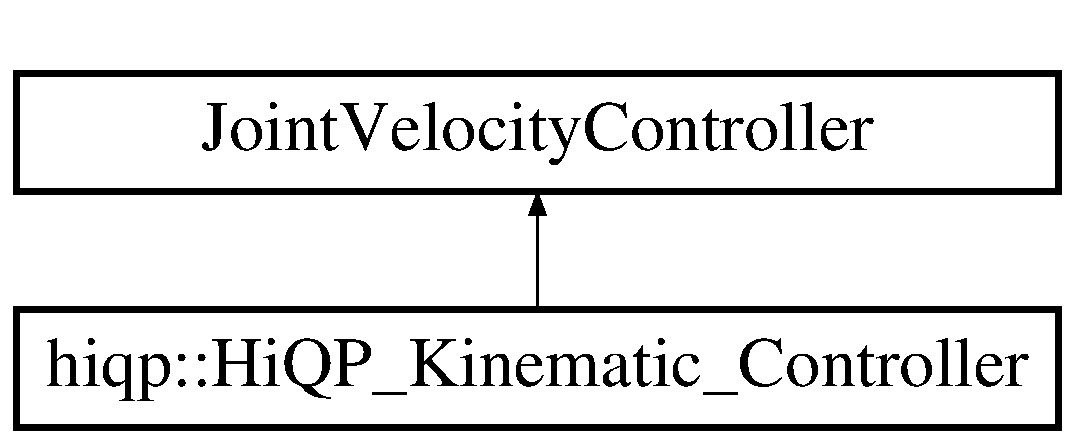
\includegraphics[height=2.000000cm]{classhiqp_1_1HiQP__Kinematic__Controller}
\end{center}
\end{figure}
\subsection*{Public Member Functions}
\begin{DoxyCompactItemize}
\item 
\hypertarget{classhiqp_1_1HiQP__Kinematic__Controller_aa82bda256000e7dc52fb4107bbdf62af}{\hyperlink{classhiqp_1_1HiQP__Kinematic__Controller_aa82bda256000e7dc52fb4107bbdf62af}{Hi\-Q\-P\-\_\-\-Kinematic\-\_\-\-Controller} ()}\label{classhiqp_1_1HiQP__Kinematic__Controller_aa82bda256000e7dc52fb4107bbdf62af}

\begin{DoxyCompactList}\small\item\em Constructor Constructs my awesome controller. \end{DoxyCompactList}\item 
\hypertarget{classhiqp_1_1HiQP__Kinematic__Controller_ae82482094e3e5eee72441b639fb63522}{\hyperlink{classhiqp_1_1HiQP__Kinematic__Controller_ae82482094e3e5eee72441b639fb63522}{$\sim$\-Hi\-Q\-P\-\_\-\-Kinematic\-\_\-\-Controller} () noexcept}\label{classhiqp_1_1HiQP__Kinematic__Controller_ae82482094e3e5eee72441b639fb63522}

\begin{DoxyCompactList}\small\item\em Destructor Destructs my awesome controller \-:(. \end{DoxyCompactList}\item 
bool \hyperlink{classhiqp_1_1HiQP__Kinematic__Controller_af42f14229f8f2d34e04eda97349f2fa2}{init} (\hyperlink{namespacehiqp_ac536ca3b4ba33489281fa5bec490799c}{Joint\-Velocity\-Interface} $\ast$hw, ros\-::\-Node\-Handle \&controller\-\_\-nh)
\begin{DoxyCompactList}\small\item\em Called every time the controller is initialized by the ros\-::controller\-\_\-manager. \end{DoxyCompactList}\item 
void \hyperlink{classhiqp_1_1HiQP__Kinematic__Controller_ad41772f143ec0725004baac5090eb7f1}{starting} (const ros\-::\-Time \&time)
\begin{DoxyCompactList}\small\item\em Called every time the controller is started by the ros\-::controller\-\_\-manager. \end{DoxyCompactList}\item 
void \hyperlink{classhiqp_1_1HiQP__Kinematic__Controller_ac8ae858ee94719281bd1abb9ca02aea4}{update} (const ros\-::\-Time \&time, const ros\-::\-Duration \&period)
\begin{DoxyCompactList}\small\item\em Called every time the controller is updated by the ros\-::controller\-\_\-manager. \end{DoxyCompactList}\item 
void \hyperlink{classhiqp_1_1HiQP__Kinematic__Controller_a7b85b552fe4923cc2fe6363efaf0a414}{stopping} (const ros\-::\-Time \&time)
\begin{DoxyCompactList}\small\item\em Called every time the controller is stopped by the ros\-::controller\-\_\-manager. \end{DoxyCompactList}\end{DoxyCompactItemize}


\subsection{Detailed Description}
This is my awesome controller. 

It's awesome! 

\subsection{Member Function Documentation}
\hypertarget{classhiqp_1_1HiQP__Kinematic__Controller_af42f14229f8f2d34e04eda97349f2fa2}{\index{hiqp\-::\-Hi\-Q\-P\-\_\-\-Kinematic\-\_\-\-Controller@{hiqp\-::\-Hi\-Q\-P\-\_\-\-Kinematic\-\_\-\-Controller}!init@{init}}
\index{init@{init}!hiqp::HiQP_Kinematic_Controller@{hiqp\-::\-Hi\-Q\-P\-\_\-\-Kinematic\-\_\-\-Controller}}
\subsubsection[{init}]{\setlength{\rightskip}{0pt plus 5cm}bool hiqp\-::\-Hi\-Q\-P\-\_\-\-Kinematic\-\_\-\-Controller\-::init (
\begin{DoxyParamCaption}
\item[{{\bf Joint\-Velocity\-Interface} $\ast$}]{hw, }
\item[{ros\-::\-Node\-Handle \&}]{controller\-\_\-nh}
\end{DoxyParamCaption}
)}}\label{classhiqp_1_1HiQP__Kinematic__Controller_af42f14229f8f2d34e04eda97349f2fa2}


Called every time the controller is initialized by the ros\-::controller\-\_\-manager. 

Does some cool stuff!


\begin{DoxyParams}{Parameters}
{\em hw} & \-: a pointer to the hardware interface used by this controller \\
\hline
{\em controller\-\_\-nh} & \-: the node handle of this controller \\
\hline
\end{DoxyParams}
\begin{DoxyReturn}{Returns}
true if the initialization was successful 
\end{DoxyReturn}
\hypertarget{classhiqp_1_1HiQP__Kinematic__Controller_ad41772f143ec0725004baac5090eb7f1}{\index{hiqp\-::\-Hi\-Q\-P\-\_\-\-Kinematic\-\_\-\-Controller@{hiqp\-::\-Hi\-Q\-P\-\_\-\-Kinematic\-\_\-\-Controller}!starting@{starting}}
\index{starting@{starting}!hiqp::HiQP_Kinematic_Controller@{hiqp\-::\-Hi\-Q\-P\-\_\-\-Kinematic\-\_\-\-Controller}}
\subsubsection[{starting}]{\setlength{\rightskip}{0pt plus 5cm}void hiqp\-::\-Hi\-Q\-P\-\_\-\-Kinematic\-\_\-\-Controller\-::starting (
\begin{DoxyParamCaption}
\item[{const ros\-::\-Time \&}]{time}
\end{DoxyParamCaption}
)}}\label{classhiqp_1_1HiQP__Kinematic__Controller_ad41772f143ec0725004baac5090eb7f1}


Called every time the controller is started by the ros\-::controller\-\_\-manager. 

Does some cool stuff!


\begin{DoxyParams}{Parameters}
{\em time} & \-: the current wall-\/time in R\-O\-S \\
\hline
\end{DoxyParams}
\begin{DoxyReturn}{Returns}
true if the starting was successful 
\end{DoxyReturn}
\hypertarget{classhiqp_1_1HiQP__Kinematic__Controller_a7b85b552fe4923cc2fe6363efaf0a414}{\index{hiqp\-::\-Hi\-Q\-P\-\_\-\-Kinematic\-\_\-\-Controller@{hiqp\-::\-Hi\-Q\-P\-\_\-\-Kinematic\-\_\-\-Controller}!stopping@{stopping}}
\index{stopping@{stopping}!hiqp::HiQP_Kinematic_Controller@{hiqp\-::\-Hi\-Q\-P\-\_\-\-Kinematic\-\_\-\-Controller}}
\subsubsection[{stopping}]{\setlength{\rightskip}{0pt plus 5cm}void hiqp\-::\-Hi\-Q\-P\-\_\-\-Kinematic\-\_\-\-Controller\-::stopping (
\begin{DoxyParamCaption}
\item[{const ros\-::\-Time \&}]{time}
\end{DoxyParamCaption}
)}}\label{classhiqp_1_1HiQP__Kinematic__Controller_a7b85b552fe4923cc2fe6363efaf0a414}


Called every time the controller is stopped by the ros\-::controller\-\_\-manager. 

Does some cool stuff!


\begin{DoxyParams}{Parameters}
{\em time} & \-: the current wall-\/time in R\-O\-S \\
\hline
\end{DoxyParams}
\begin{DoxyReturn}{Returns}
true if the stopping was successful 
\end{DoxyReturn}
\hypertarget{classhiqp_1_1HiQP__Kinematic__Controller_ac8ae858ee94719281bd1abb9ca02aea4}{\index{hiqp\-::\-Hi\-Q\-P\-\_\-\-Kinematic\-\_\-\-Controller@{hiqp\-::\-Hi\-Q\-P\-\_\-\-Kinematic\-\_\-\-Controller}!update@{update}}
\index{update@{update}!hiqp::HiQP_Kinematic_Controller@{hiqp\-::\-Hi\-Q\-P\-\_\-\-Kinematic\-\_\-\-Controller}}
\subsubsection[{update}]{\setlength{\rightskip}{0pt plus 5cm}void hiqp\-::\-Hi\-Q\-P\-\_\-\-Kinematic\-\_\-\-Controller\-::update (
\begin{DoxyParamCaption}
\item[{const ros\-::\-Time \&}]{time, }
\item[{const ros\-::\-Duration \&}]{period}
\end{DoxyParamCaption}
)}}\label{classhiqp_1_1HiQP__Kinematic__Controller_ac8ae858ee94719281bd1abb9ca02aea4}


Called every time the controller is updated by the ros\-::controller\-\_\-manager. 

Does some cool stuff!


\begin{DoxyParams}{Parameters}
{\em time} & \-: the current wall-\/time in R\-O\-S \\
\hline
{\em period} & \-: the time between the last update call and this, i.\-e. the sample time. \\
\hline
\end{DoxyParams}
\begin{DoxyReturn}{Returns}
true if the update was successful 
\end{DoxyReturn}


The documentation for this class was generated from the following files\-:\begin{DoxyCompactItemize}
\item 
include/hiqp\-\_\-kinematic\-\_\-controller.\-h\item 
src/hiqp\-\_\-kinematic\-\_\-controller.\-cpp\end{DoxyCompactItemize}

\hypertarget{classhiqp_1_1Task}{\section{hiqp\-:\-:Task Class Reference}
\label{classhiqp_1_1Task}\index{hiqp\-::\-Task@{hiqp\-::\-Task}}
}
Inheritance diagram for hiqp\-:\-:Task\-:\begin{figure}[H]
\begin{center}
\leavevmode
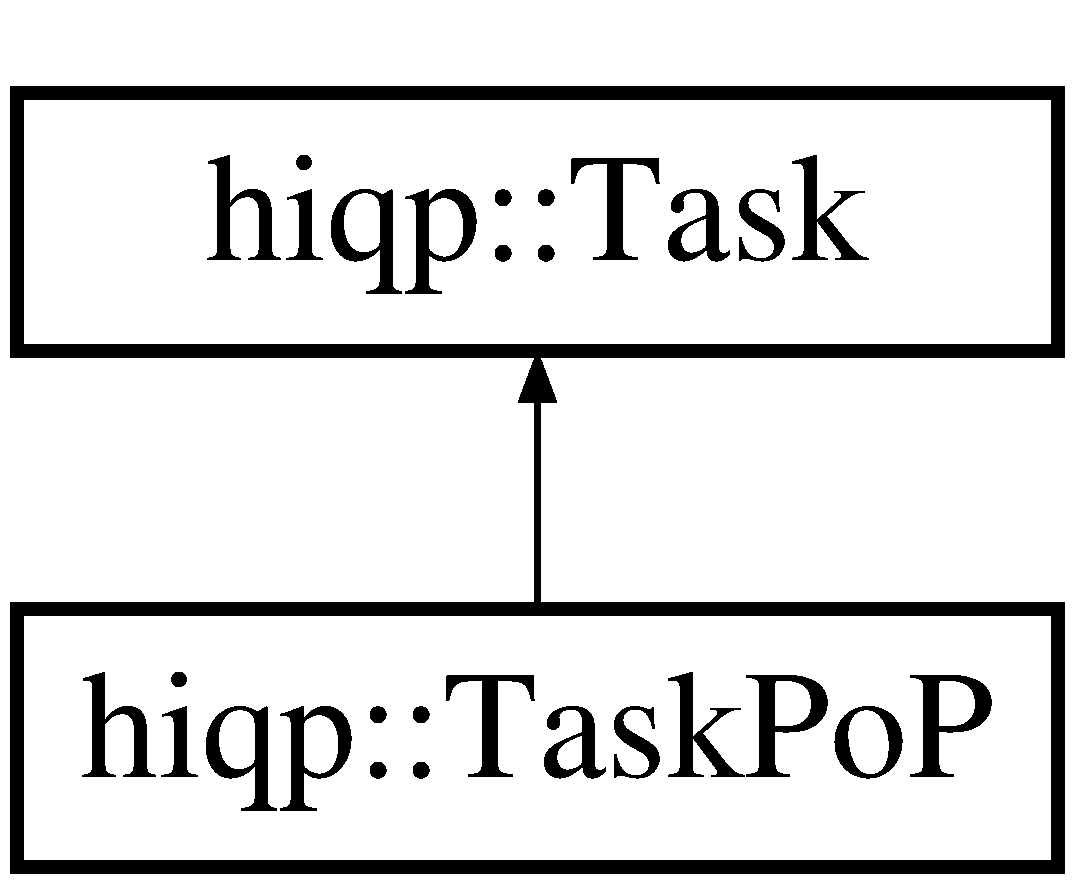
\includegraphics[height=2.000000cm]{classhiqp_1_1Task}
\end{center}
\end{figure}
\subsection*{Public Member Functions}
\begin{DoxyCompactItemize}
\item 
\hypertarget{classhiqp_1_1Task_a556692dacc6abb51d0437f59594026d9}{\hyperlink{classhiqp_1_1Task_a556692dacc6abb51d0437f59594026d9}{Task} ()}\label{classhiqp_1_1Task_a556692dacc6abb51d0437f59594026d9}

\begin{DoxyCompactList}\small\item\em Constructor Constructs my awesome task. \end{DoxyCompactList}\item 
\hypertarget{classhiqp_1_1Task_a73b4e41812713f28557c8d15925587db}{\hyperlink{classhiqp_1_1Task_a73b4e41812713f28557c8d15925587db}{$\sim$\-Task} () noexcept}\label{classhiqp_1_1Task_a73b4e41812713f28557c8d15925587db}

\begin{DoxyCompactList}\small\item\em Destructor Destructs my awesome task. \end{DoxyCompactList}\item 
\hypertarget{classhiqp_1_1Task_a02b6ccead41f86f26e7d1b2cb2e013ae}{virtual int {\bfseries init} (const std\-::vector$<$ std\-::string $>$ \&parameters)=0}\label{classhiqp_1_1Task_a02b6ccead41f86f26e7d1b2cb2e013ae}

\item 
virtual int \hyperlink{classhiqp_1_1Task_a2f81c249b39a1fd6557501d61548917b}{apply} (const K\-D\-L\-::\-Tree \&kdl\-\_\-tree, const K\-D\-L\-::\-Jnt\-Array\-Vel \&kdl\-\_\-joint\-\_\-pos\-\_\-vel)=0
\begin{DoxyCompactList}\small\item\em {\itshape Pure virtual}. Calculates the task function and task jacobian values. \end{DoxyCompactList}\item 
\hypertarget{classhiqp_1_1Task_a0d018a8a797cb730111614a9230d59e2}{virtual int {\bfseries draw} ()=0}\label{classhiqp_1_1Task_a0d018a8a797cb730111614a9230d59e2}

\end{DoxyCompactItemize}
\subsection*{Protected Member Functions}
\begin{DoxyCompactItemize}
\item 
\hypertarget{classhiqp_1_1Task_adbd4a69acbd2402d14fc51446d9c7a94}{\hyperlink{classhiqp_1_1TaskVisualizer}{Task\-Visualizer} $\ast$ {\bfseries get\-Task\-Visualizer} ()}\label{classhiqp_1_1Task_adbd4a69acbd2402d14fc51446d9c7a94}

\end{DoxyCompactItemize}
\subsection*{Protected Attributes}
\begin{DoxyCompactItemize}
\item 
\hypertarget{classhiqp_1_1Task_af1290bb9764f71d8abd3c26eb6997425}{double {\bfseries e\-\_\-}}\label{classhiqp_1_1Task_af1290bb9764f71d8abd3c26eb6997425}

\item 
\hypertarget{classhiqp_1_1Task_a10cc3261be638fbc5778c1ee71c16784}{Eigen\-::\-Matrix\-Xd {\bfseries J\-\_\-}}\label{classhiqp_1_1Task_a10cc3261be638fbc5778c1ee71c16784}

\end{DoxyCompactItemize}


\subsection{Member Function Documentation}
\hypertarget{classhiqp_1_1Task_a2f81c249b39a1fd6557501d61548917b}{\index{hiqp\-::\-Task@{hiqp\-::\-Task}!apply@{apply}}
\index{apply@{apply}!hiqp::Task@{hiqp\-::\-Task}}
\subsubsection[{apply}]{\setlength{\rightskip}{0pt plus 5cm}virtual int hiqp\-::\-Task\-::apply (
\begin{DoxyParamCaption}
\item[{const K\-D\-L\-::\-Tree \&}]{kdl\-\_\-tree, }
\item[{const K\-D\-L\-::\-Jnt\-Array\-Vel \&}]{kdl\-\_\-joint\-\_\-pos\-\_\-vel}
\end{DoxyParamCaption}
)\hspace{0.3cm}{\ttfamily [pure virtual]}}}\label{classhiqp_1_1Task_a2f81c249b39a1fd6557501d61548917b}


{\itshape Pure virtual}. Calculates the task function and task jacobian values. 


\begin{DoxyParams}{Parameters}
{\em kdl\-\_\-tree} & \-: reference to the kinematic dynamic tree of the robot \\
\hline
{\em kdl\-\_\-joint\-\_\-pos\-\_\-vel} & \-: reference to the current joint positions and velocities \\
\hline
{\em task\-\_\-fun\-\_\-val} & \-: reference to where the output controls are to be stored\\
\hline
\end{DoxyParams}
\begin{DoxyReturn}{Returns}
0 if the calculation was successful 
\end{DoxyReturn}


Implemented in \hyperlink{classhiqp_1_1TaskPoP_a7f50f65c7e09492a0021715ad2ef2866}{hiqp\-::\-Task\-Po\-P}.



The documentation for this class was generated from the following file\-:\begin{DoxyCompactItemize}
\item 
include/hiqp/\hyperlink{task_8h}{task.\-h}\end{DoxyCompactItemize}

\hypertarget{classhiqp_1_1TaskManager}{\section{hiqp\-:\-:Task\-Manager Class Reference}
\label{classhiqp_1_1TaskManager}\index{hiqp\-::\-Task\-Manager@{hiqp\-::\-Task\-Manager}}
}


Should be created only once!  




{\ttfamily \#include $<$task\-\_\-manager.\-h$>$}

\subsection*{Public Member Functions}
\begin{DoxyCompactItemize}
\item 
\hypertarget{classhiqp_1_1TaskManager_af190d8f0b3ee1c0d32acdb70fae6e03d}{\hyperlink{classhiqp_1_1TaskManager_af190d8f0b3ee1c0d32acdb70fae6e03d}{Task\-Manager} ()}\label{classhiqp_1_1TaskManager_af190d8f0b3ee1c0d32acdb70fae6e03d}

\begin{DoxyCompactList}\small\item\em Constructor Constructs my awesome controller. \end{DoxyCompactList}\item 
\hypertarget{classhiqp_1_1TaskManager_a688ad548e2ef681b458c1fc90326f6e6}{\hyperlink{classhiqp_1_1TaskManager_a688ad548e2ef681b458c1fc90326f6e6}{$\sim$\-Task\-Manager} () noexcept}\label{classhiqp_1_1TaskManager_a688ad548e2ef681b458c1fc90326f6e6}

\begin{DoxyCompactList}\small\item\em Destructor Destructs my awesome manager. \end{DoxyCompactList}\item 
bool \hyperlink{classhiqp_1_1TaskManager_a9243435c3819b03a9874f47d985a2147}{get\-Kinematic\-Controls} (const K\-D\-L\-::\-Tree \&kdl\-\_\-tree, const K\-D\-L\-::\-Jnt\-Array\-Vel \&kdl\-\_\-joint\-\_\-pos\-\_\-vel, unsigned int n\-\_\-controls, std\-::vector$<$ double $>$ \&controls)
\begin{DoxyCompactList}\small\item\em Called every time the controller is initialized by the ros\-::controller\-\_\-manager. \end{DoxyCompactList}\end{DoxyCompactItemize}


\subsection{Detailed Description}
Should be created only once! 

It's awesome! 

\subsection{Member Function Documentation}
\hypertarget{classhiqp_1_1TaskManager_a9243435c3819b03a9874f47d985a2147}{\index{hiqp\-::\-Task\-Manager@{hiqp\-::\-Task\-Manager}!get\-Kinematic\-Controls@{get\-Kinematic\-Controls}}
\index{get\-Kinematic\-Controls@{get\-Kinematic\-Controls}!hiqp::TaskManager@{hiqp\-::\-Task\-Manager}}
\subsubsection[{get\-Kinematic\-Controls}]{\setlength{\rightskip}{0pt plus 5cm}bool hiqp\-::\-Task\-Manager\-::get\-Kinematic\-Controls (
\begin{DoxyParamCaption}
\item[{const K\-D\-L\-::\-Tree \&}]{kdl\-\_\-tree, }
\item[{const K\-D\-L\-::\-Jnt\-Array\-Vel \&}]{kdl\-\_\-joint\-\_\-pos\-\_\-vel, }
\item[{unsigned int}]{n\-\_\-controls, }
\item[{std\-::vector$<$ double $>$ \&}]{controls}
\end{DoxyParamCaption}
)}}\label{classhiqp_1_1TaskManager_a9243435c3819b03a9874f47d985a2147}


Called every time the controller is initialized by the ros\-::controller\-\_\-manager. 

Does some cool stuff!


\begin{DoxyParams}{Parameters}
{\em kdl\-\_\-tree} & \-: the kinematic dynamic tree of the robot \\
\hline
{\em n\-\_\-controls} & \-: the number of controls \\
\hline
{\em controls} & \-: reference to the controls data \\
\hline
\end{DoxyParams}
\begin{DoxyReturn}{Returns}
true if the initialization was successful 
\end{DoxyReturn}


The documentation for this class was generated from the following files\-:\begin{DoxyCompactItemize}
\item 
include/\hyperlink{task__manager_8h}{task\-\_\-manager.\-h}\item 
src/task\-\_\-manager.\-cpp\end{DoxyCompactItemize}

\chapter{File Documentation}
\hypertarget{task_8h}{\section{include/hiqp/task.h File Reference}
\label{task_8h}\index{include/hiqp/task.\-h@{include/hiqp/task.\-h}}
}


Brief description of file.  


{\ttfamily \#include $<$hiqp/task\-\_\-behaviour.\-h$>$}\\*
{\ttfamily \#include $<$hiqp/task\-\_\-visualizer.\-h$>$}\\*
{\ttfamily \#include $<$vector$>$}\\*
{\ttfamily \#include $<$iostream$>$}\\*
{\ttfamily \#include $<$Eigen/\-Dense$>$}\\*
{\ttfamily \#include $<$kdl/tree.\-hpp$>$}\\*
{\ttfamily \#include $<$kdl/jntarrayvel.\-hpp$>$}\\*
\subsection*{Classes}
\begin{DoxyCompactItemize}
\item 
class \hyperlink{classhiqp_1_1Task}{hiqp\-::\-Task}
\end{DoxyCompactItemize}
\subsection*{Namespaces}
\begin{DoxyCompactItemize}
\item 
\hyperlink{namespacehiqp}{hiqp}
\end{DoxyCompactItemize}


\subsection{Detailed Description}
Brief description of file. Marcus A Johansson (\href{mailto:marcus.adam.johansson@gmail.com}{\tt marcus.\-adam.\-johansson@gmail.\-com}) \begin{DoxyDate}{Date}
July, 2016 Detailed description of file. 
\end{DoxyDate}

\hypertarget{task__manager_8h}{\section{include/task\-\_\-manager.h File Reference}
\label{task__manager_8h}\index{include/task\-\_\-manager.\-h@{include/task\-\_\-manager.\-h}}
}


A manager class that provides an interface to all tasks.  


{\ttfamily \#include $<$vector$>$}\\*
{\ttfamily \#include $<$kdl/tree.\-hpp$>$}\\*
{\ttfamily \#include $<$kdl/jntarray.\-hpp$>$}\\*
{\ttfamily \#include $<$kdl/jntarrayvel.\-hpp$>$}\\*
\subsection*{Classes}
\begin{DoxyCompactItemize}
\item 
class \hyperlink{classhiqp_1_1TaskManager}{hiqp\-::\-Task\-Manager}
\begin{DoxyCompactList}\small\item\em Should be created only once! \end{DoxyCompactList}\end{DoxyCompactItemize}
\subsection*{Namespaces}
\begin{DoxyCompactItemize}
\item 
\hyperlink{namespacehiqp}{hiqp}
\end{DoxyCompactItemize}


\subsection{Detailed Description}
A manager class that provides an interface to all tasks. \begin{DoxyAuthor}{Author}
Marcus A Johansson 
\end{DoxyAuthor}
\begin{DoxyVersion}{Version}
0.\-1 
\end{DoxyVersion}
\begin{DoxyDate}{Date}
2016-\/06-\/28 
\end{DoxyDate}

%--- End generated contents ---

% Index
\newpage
\phantomsection
\addcontentsline{toc}{chapter}{Index}
\printindex

\end{document}
